\documentclass[main.tex]{subfiles}

\begin{document}
\section{Na Sinaji objevili skalní malby staré až 10 000 let}
Nejsme tak odlišní od lidí minulosti. Zatímco vy dnes scrollujete zdí na sockách a~koukáte při tom na nej(h)různější domácí i~světové novinky, skalní formace na Sinajském poloostrově byla čímsi takovým v~uplynulých 10 tisíci letech. Vědátoři totiž odkryli rozsáhlé naleziště skalního umění, do něhož se v~průběhu epoch podepisovaly různé kultury.
\subsection*{10 tisíc let lidských „statusů“}
\begin{wrapfigure}{r}{0.4\linewidth}
  \centering
  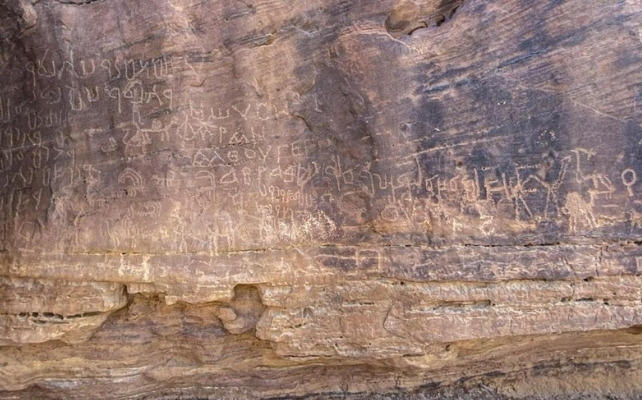
\includegraphics[width=0.95\linewidth]{sinaj1.png}
\end{wrapfigure}
Asi nejvíce zarazí nejstarší vrstvy, které mohou být staré až 10 000 let – jenom pro ilustraci, Cheopsova pyramida je blíže naší dnešní době než těmto prastarým čáranicím. Tyto nejstarší malby patrně pocházejí z~období pozdního paleolitu či raného neolitu, kdy se klima severní Afriky postupně měnilo a~oblast byla vlhčí než dnes.\par
Skála je však pokrytá rytinami a~malbami i~z různých dalších historických období – od pravěku až po islámskou éru. To znamená, že místo nebylo jednorázovou galerií, ale dlouhodobě využívaným „komunikačním panelem“ generací poutníků, pastevců a~obchodníků.
\subsection*{Skála jako kronika}
Lokalita se nachází na náhorní plošině Umm Irák a~tvoří ji přibližně sto metrů dlouhý skalní převis. Jeho strop zdobí zejména červeně malovaná zvířata a~symboly – ty jsou paradoxně těmi nejstaršími. Použití červeného pigmentu (pravděpodobně okru) je pro pravěké umění typické a~jeho dochování naznačuje, že převis poskytoval relativně stabilní mikroklima.\par
K těmto vrstvám se postupně přidaly mladší nápisy v~nabatejštině a~arabštině, což dokládá, že místo bylo využíváno a~navštěvováno po tisíciletí později různými kulturami. Nabatejci byli významnými obchodníky v~oblasti mezi 1. stoletím př. n. l. a~1. stoletím n. l., takže převis mohl ležet poblíž dávných obchodních tras spojujících Arabský poloostrov s~Levantou a~Egyptem.
\subsection*{Úkryt i~symbolické místo}
\begin{wrapfigure}{r}{0.4\linewidth}
  \centering
  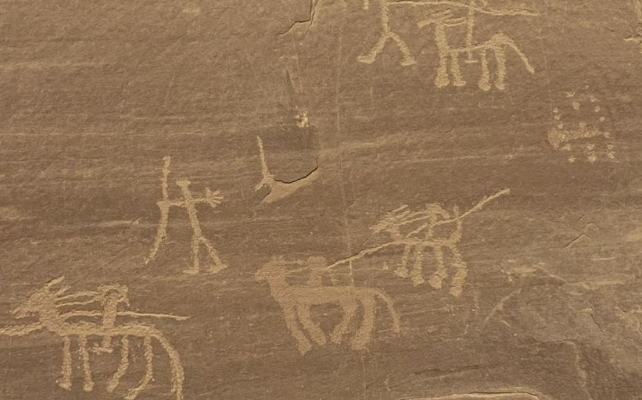
\includegraphics[width=0.95\linewidth]{sinaj2.png}
\end{wrapfigure}
Podle egyptských památkářů skála představuje jakési „přírodní muzeum pod širým nebem“, kde lze sledovat proměny lidského uměleckého projevu i~způsobu života. Archeologické nálezy uvnitř převisu – zvířecí trus, zbytky ohnišť či opracované kameny – naznačují, že lokalita nesloužila jen jako místo rituální či symbolické, ale také jako dlouhodobý úkryt.\par
Některé rytiny zachycují hospodářské aktivity prvních lidských společenství – zvířata, pastevecké motivy či symbolické značky – a~poskytují cenné informace o~každodenním životě tehdejších obyvatel. Na detailní analýzu vrstev, datování pigmentů i~přesné kulturní přiřazení si však budeme muset ještě posečkat.
\subsection*{Závod s~turismem}
Lokalita je nicméně relevantní i~dnes. Jižní část Sinaje, kde se nachází, totiž prochází rozsáhlým turistickým rozvojem v~oblasti hory svaté Kateřiny – významného křesťanského poutního místa.\par
Archeologové proto musí místo rychle zdokumentovat a~detailně prozkoumat ještě před zahájením plánovaných stavebních prací a~pravděpodobným přívalem turistů. Skalní převis tak možná čeká další kapitola – tentokrát už ne pravěká, ale moderní, ve které půjde o~ochranu toho, co tu lidé zanechávali po deset tisíc let. Poslední příběh téhle skalní formace se tak možná teprve začal psát…
\newpage
\end{document}